% lampiran.tex

\cleardoublepage

% Halaman judul "LAMPIRAN" (Aturan No. 3)
\thispagestyle{empty}
\vspace*{\fill}
\begin{center}
    \huge\bfseries LAMPIRAN
\end{center}
\vfill
\cleardoublepage

% Reset counter lampiran ke alfabet (A, B, C...)
\setcounter{lampiran}{0}

% lampiran.tex

\mulailampiran{Dokumentasi Kegiatan Magang}
    % Baris pertama (2 foto berjajar)
    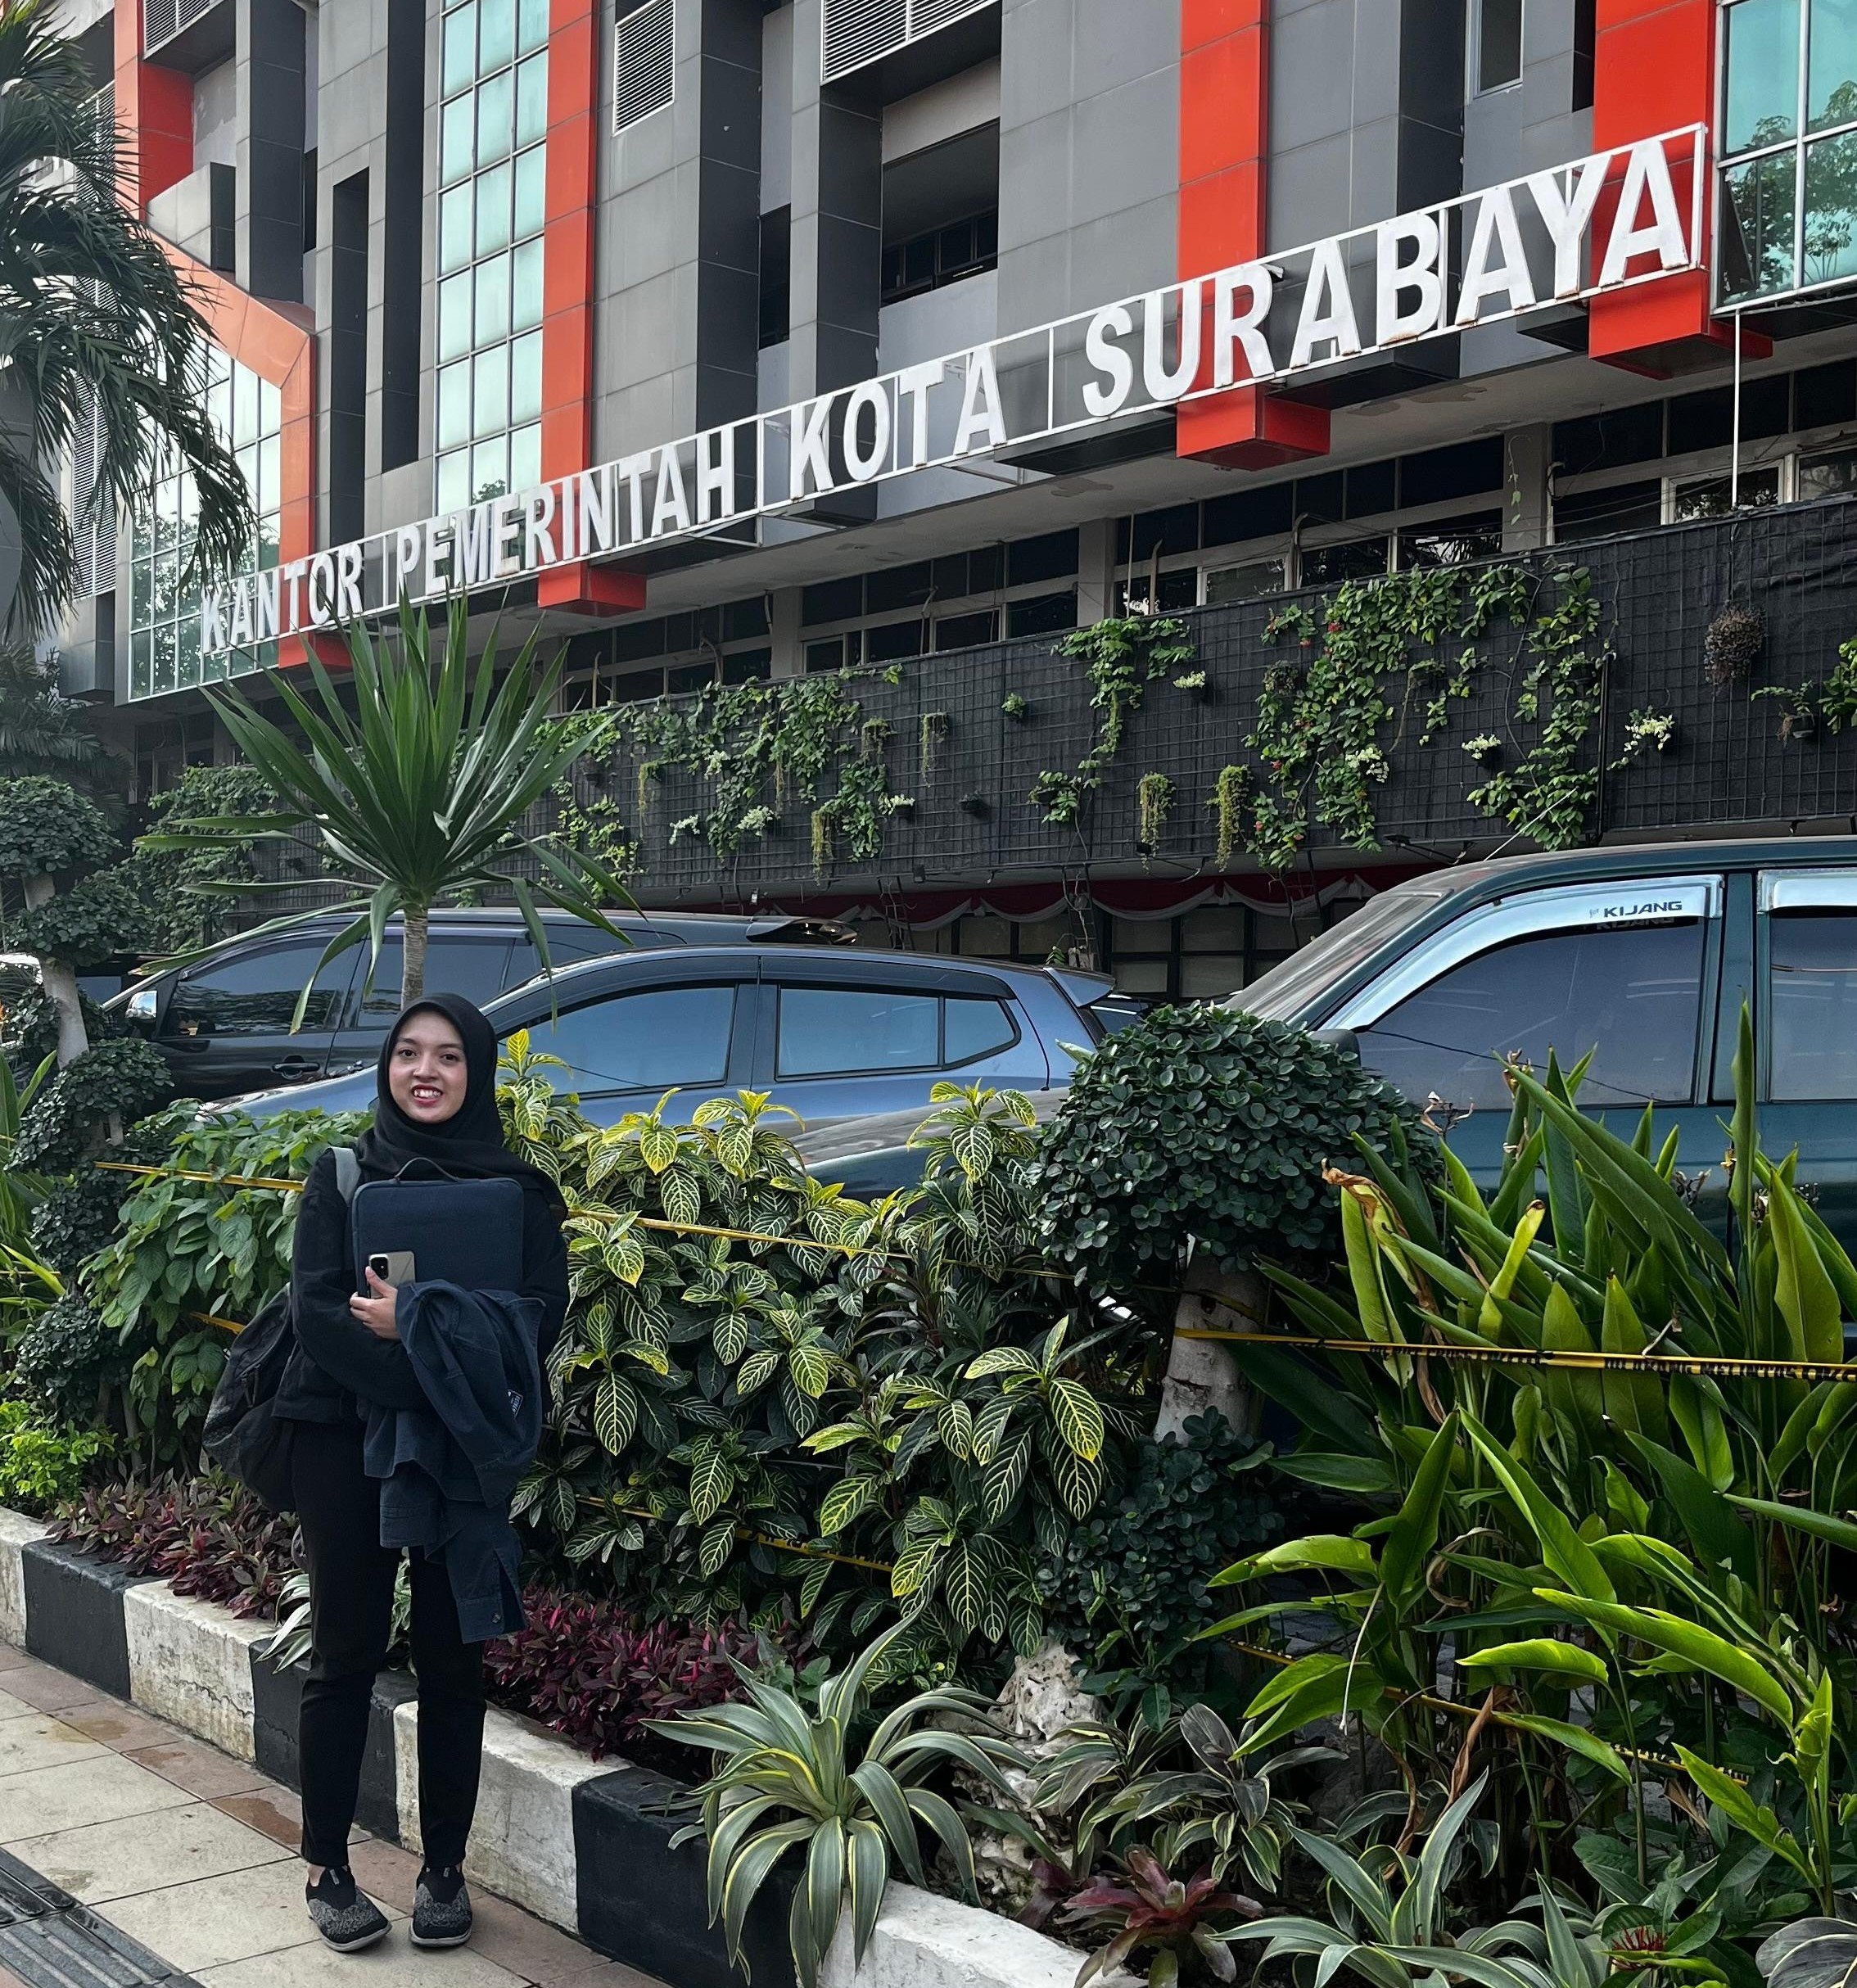
\includegraphics[width=0.5\textwidth]{gambar/dokumentasi/dokumentasi-3.jpg} \hfill
    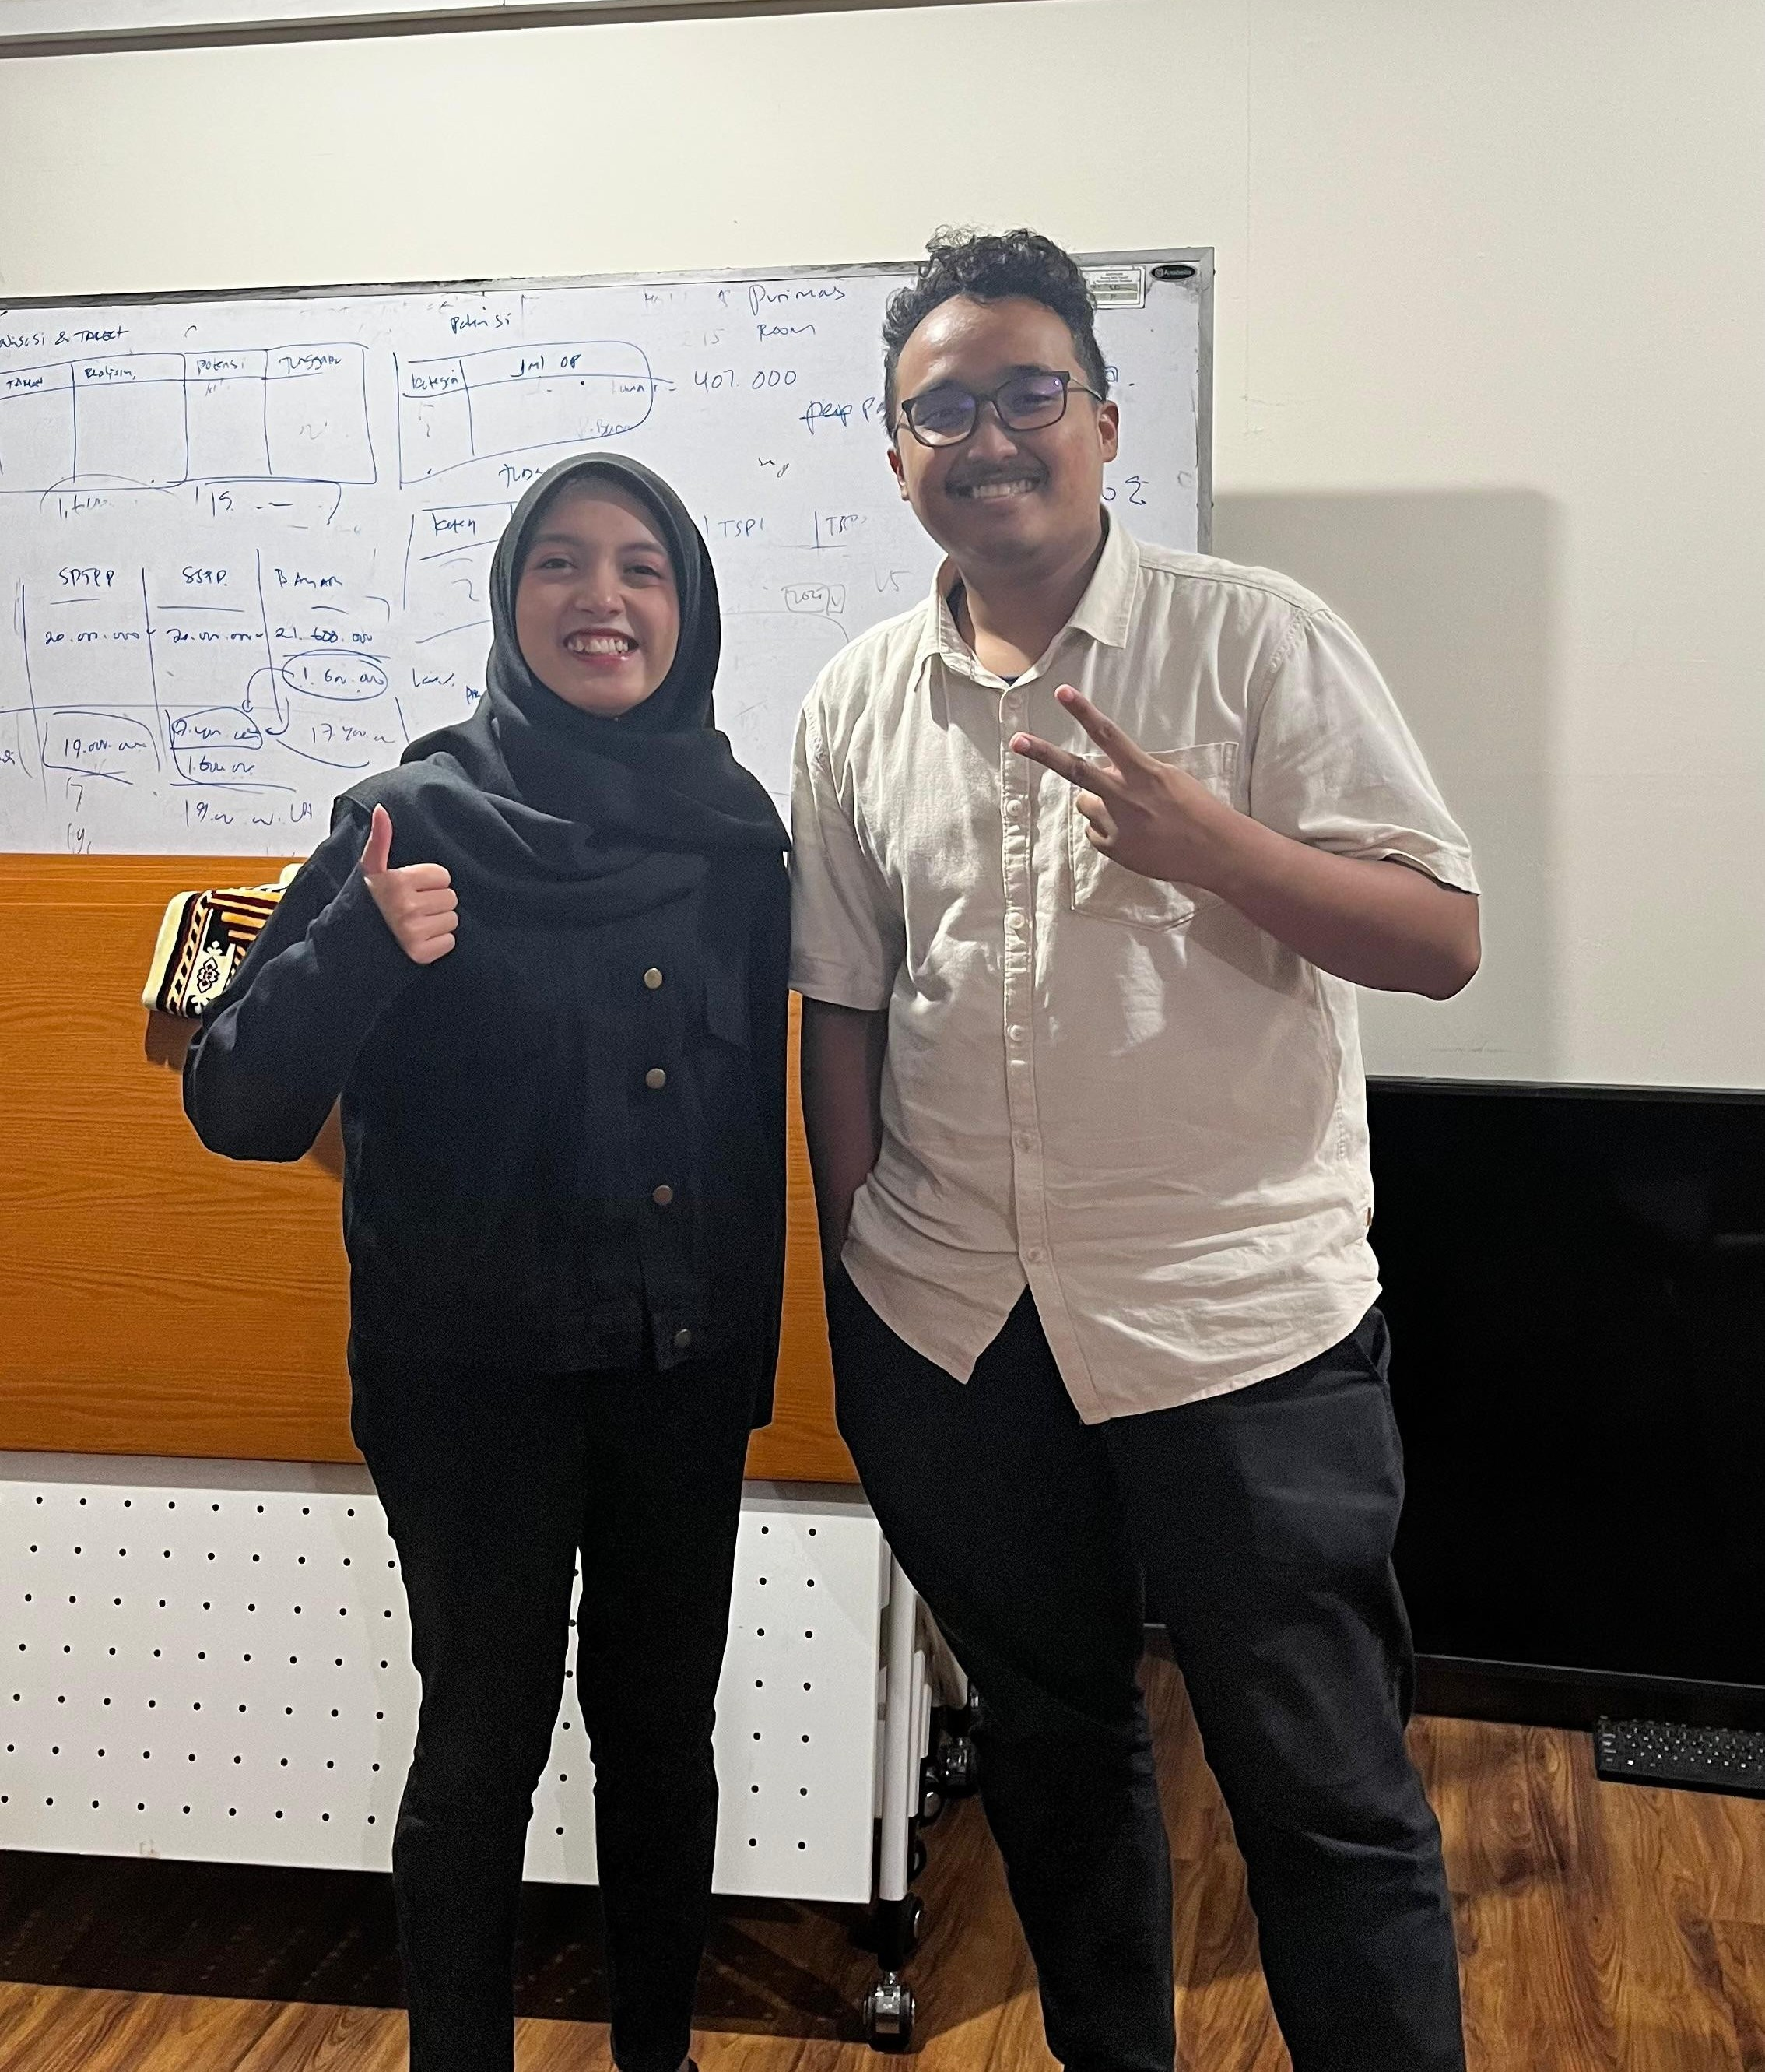
\includegraphics[width=0.48\textwidth]{gambar/dokumentasi/dokumentasi-2.jpg} 
    
    \vspace{0.5cm} % Jarak vertikal antar foto
    
    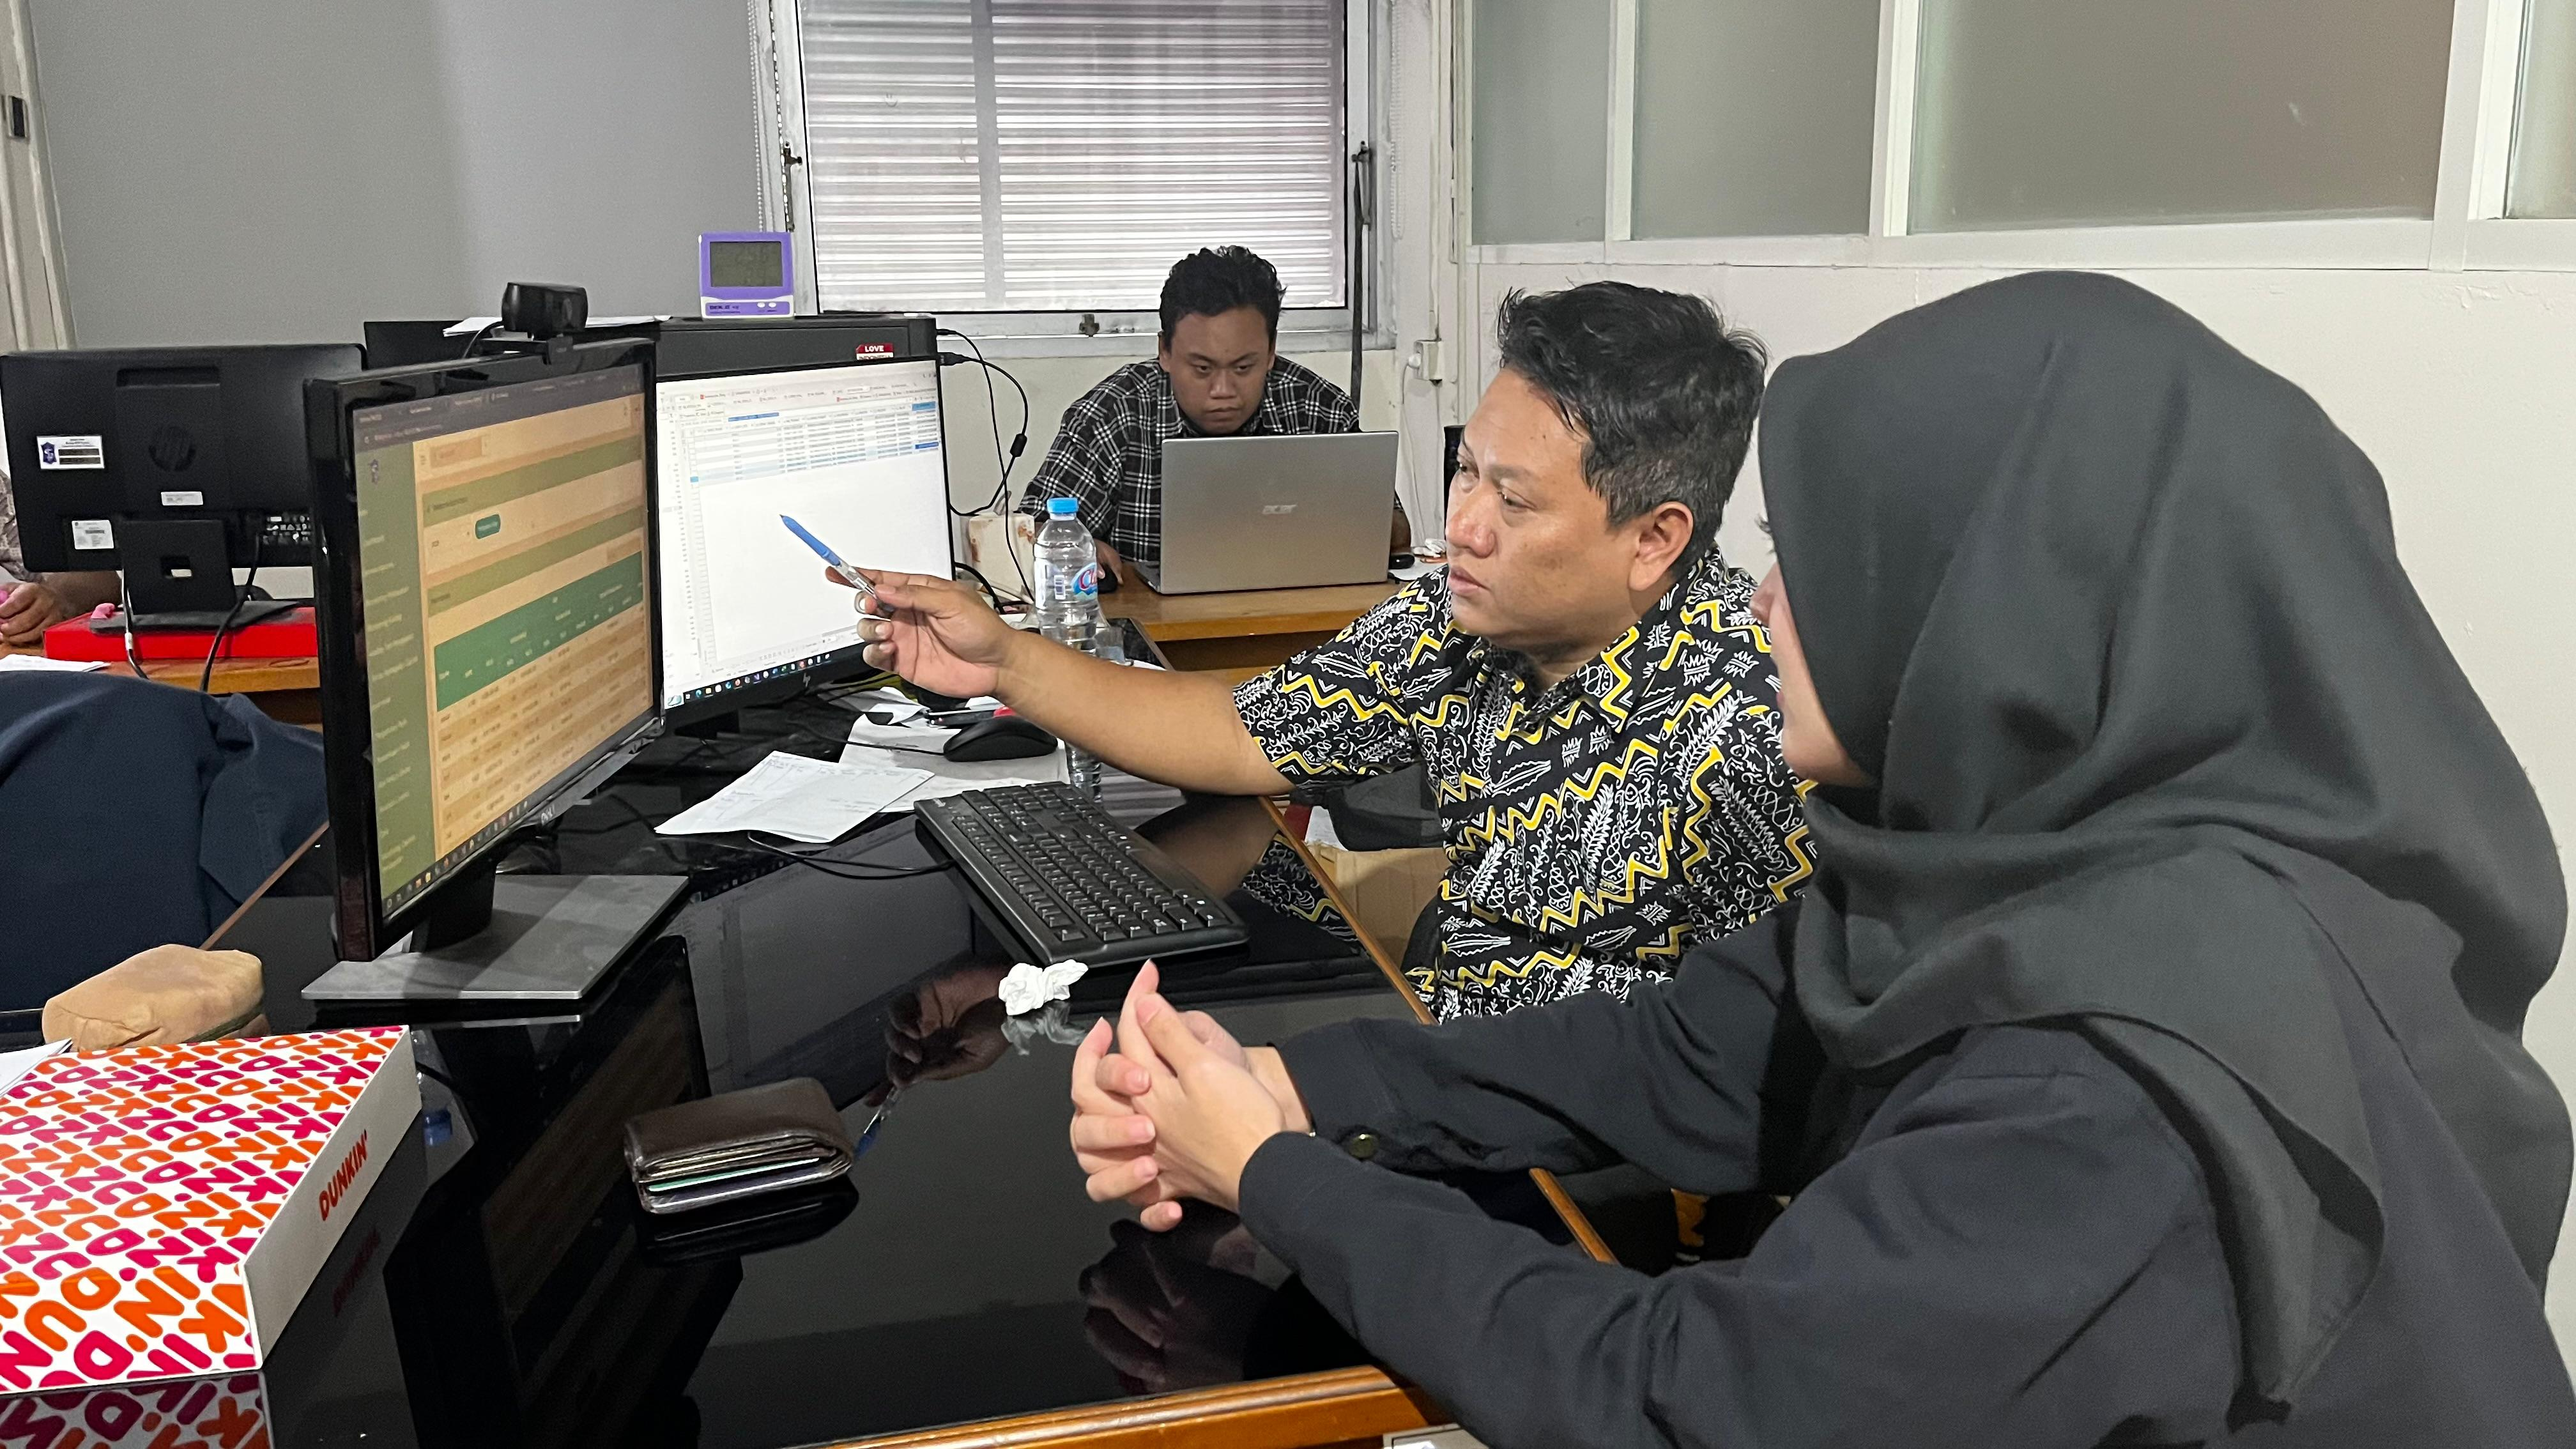
\includegraphics[width=0.9\textwidth]{gambar/dokumentasi/dokumentasi-1.jpg} \hfill
\tutuplampiran

\mulailampiran{Surat Keterangan Selesai Magang}
    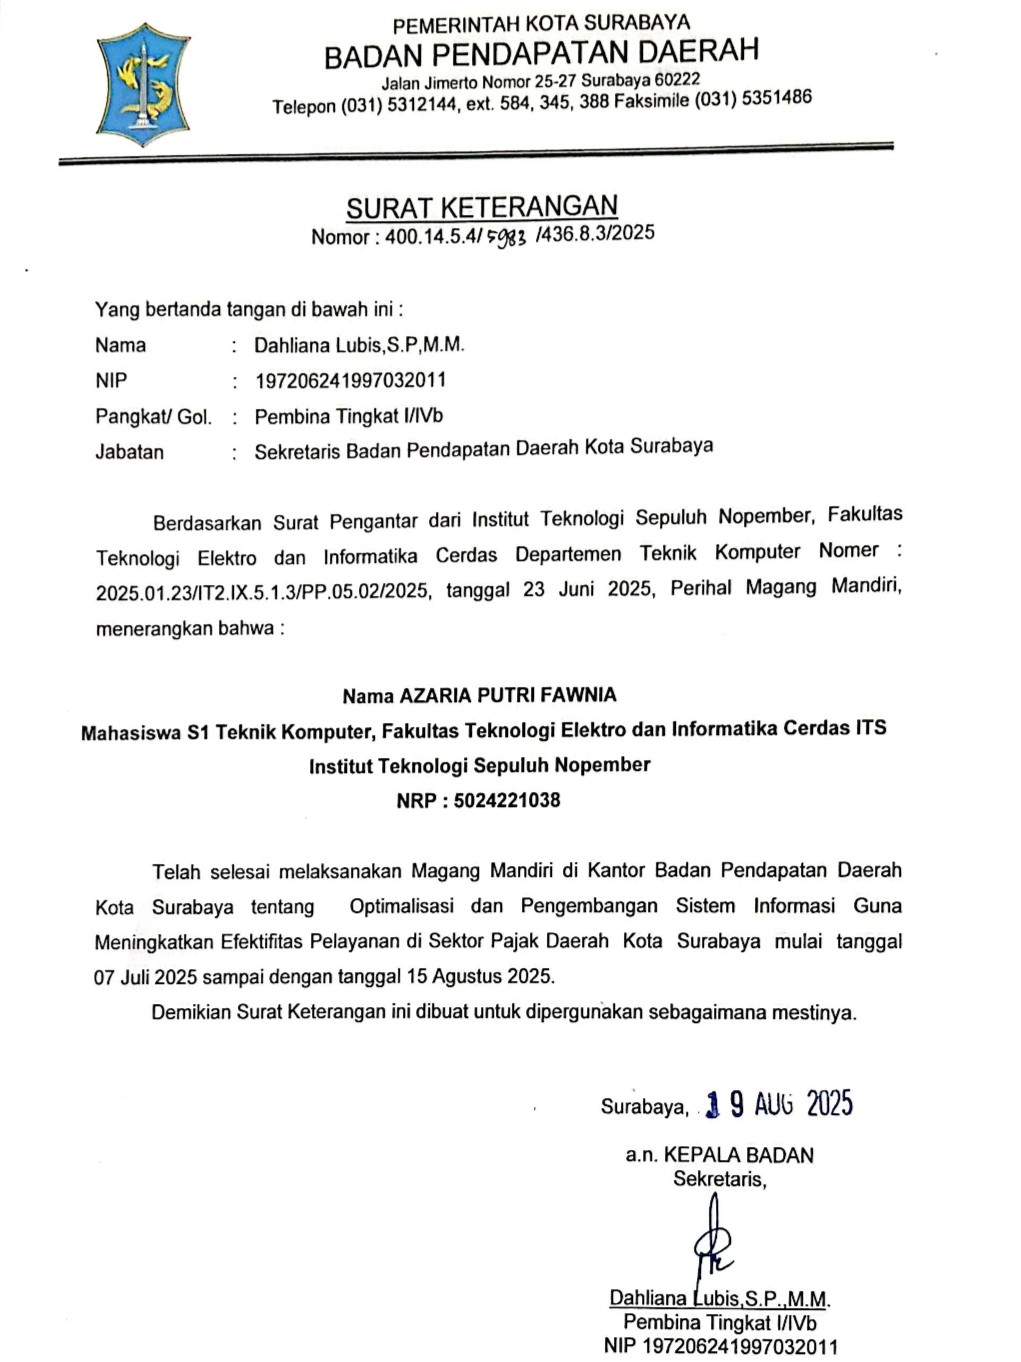
\includegraphics[width=0.95\textwidth]{gambar/surat-keterangan-selesai-magang.jpg} \hfill    
\tutuplampiran

\mulailampiran{Lembar Penilaian Kinerja Magang}
    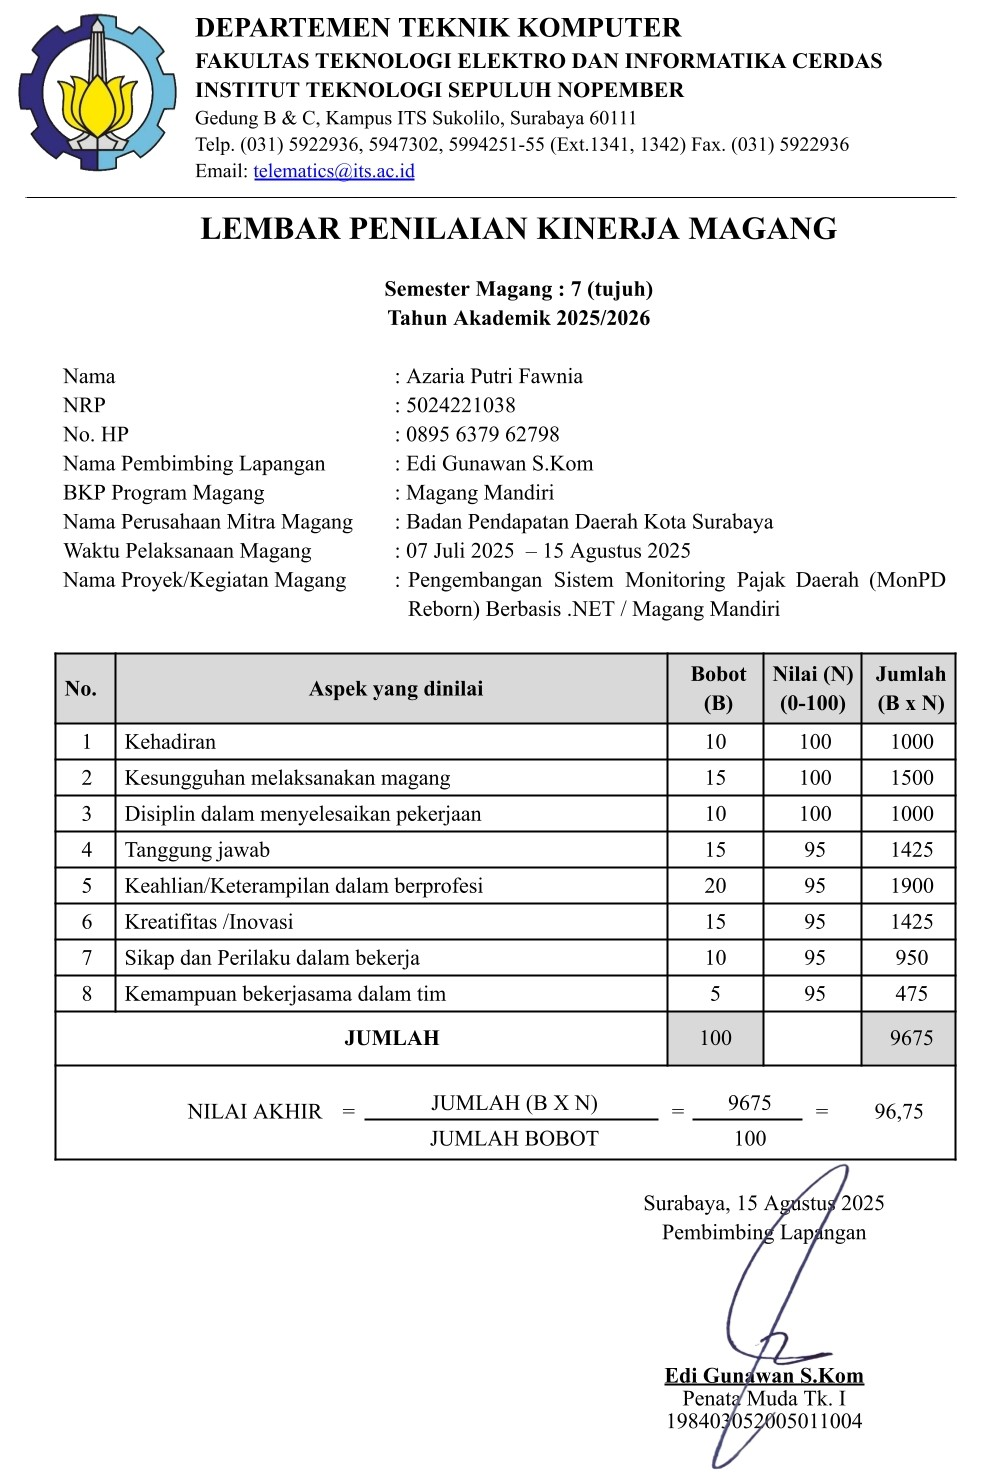
\includegraphics[width=0.92\textwidth]{gambar/penilaian-bapenda.jpg} \hfill    
\tutuplampiran

\mulailampiran{Logbook Kegiatan Magang}
    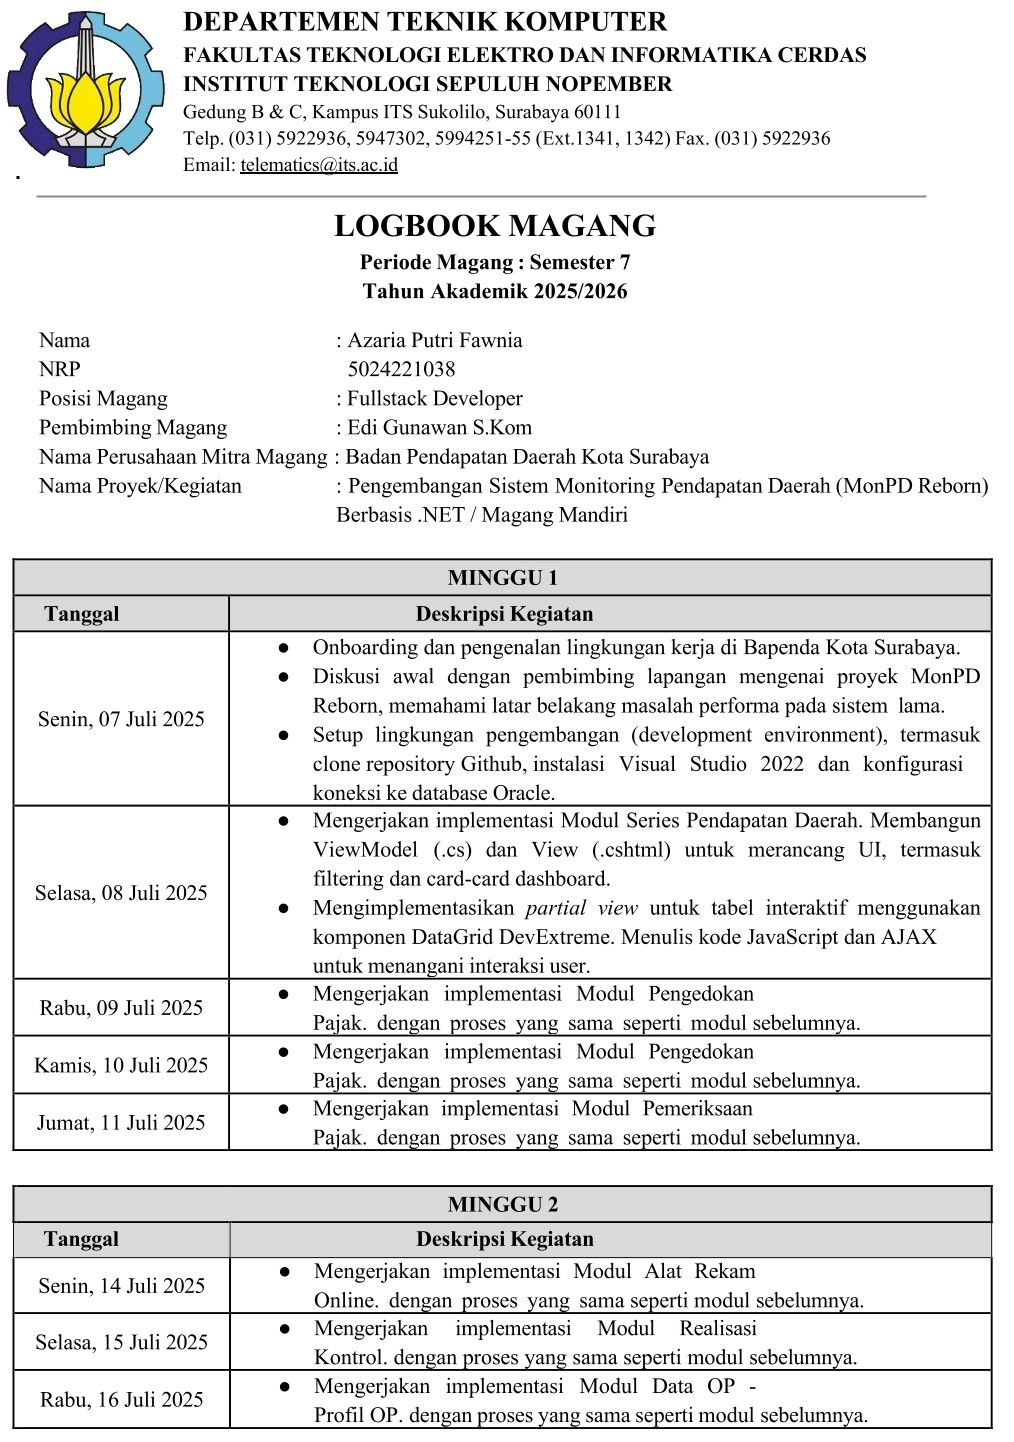
\includegraphics[width=0.96\textwidth]{gambar/logbook/Logbook-1.jpg} \hfill
    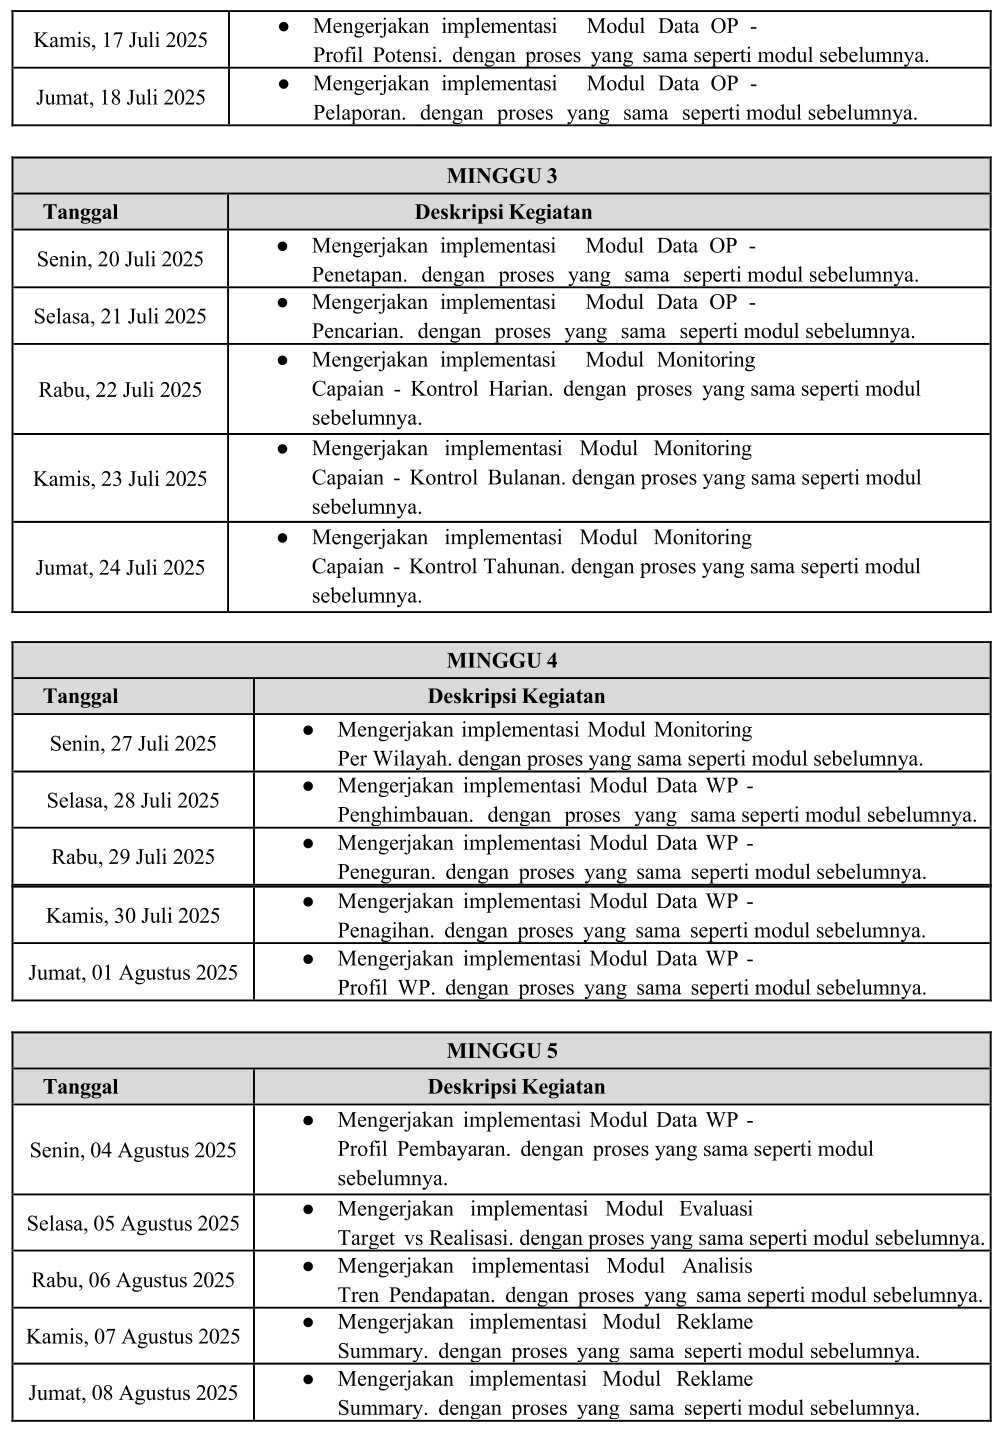
\includegraphics[width=1\textwidth]{gambar/logbook/Logbook-2.jpg} \hfill
    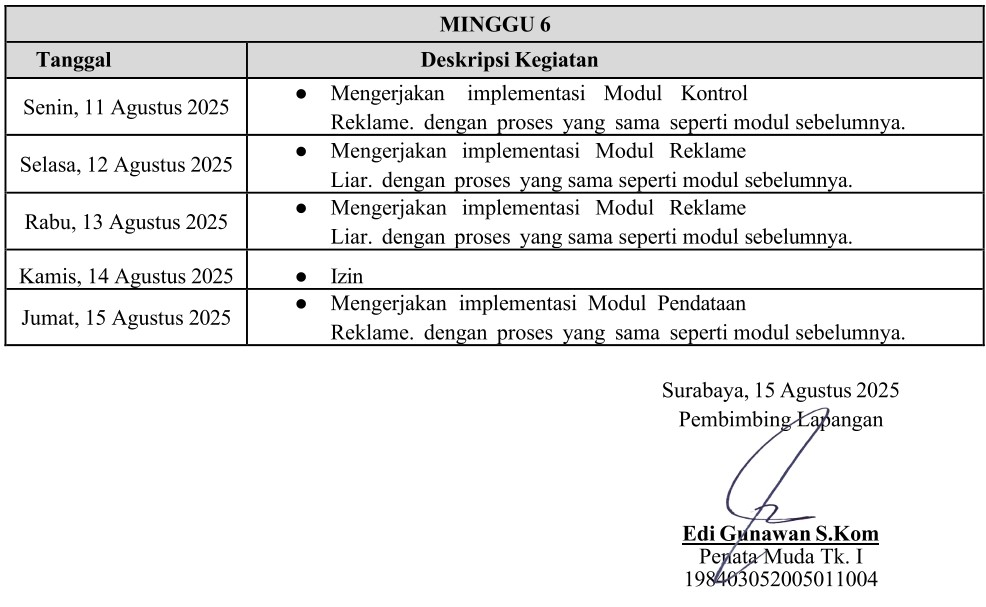
\includegraphics[width=1\textwidth]{gambar/logbook/Logbook-3.jpg} \hfill
\tutuplampiran

\mulailampiran{Presensi Kehadiran Magang}
    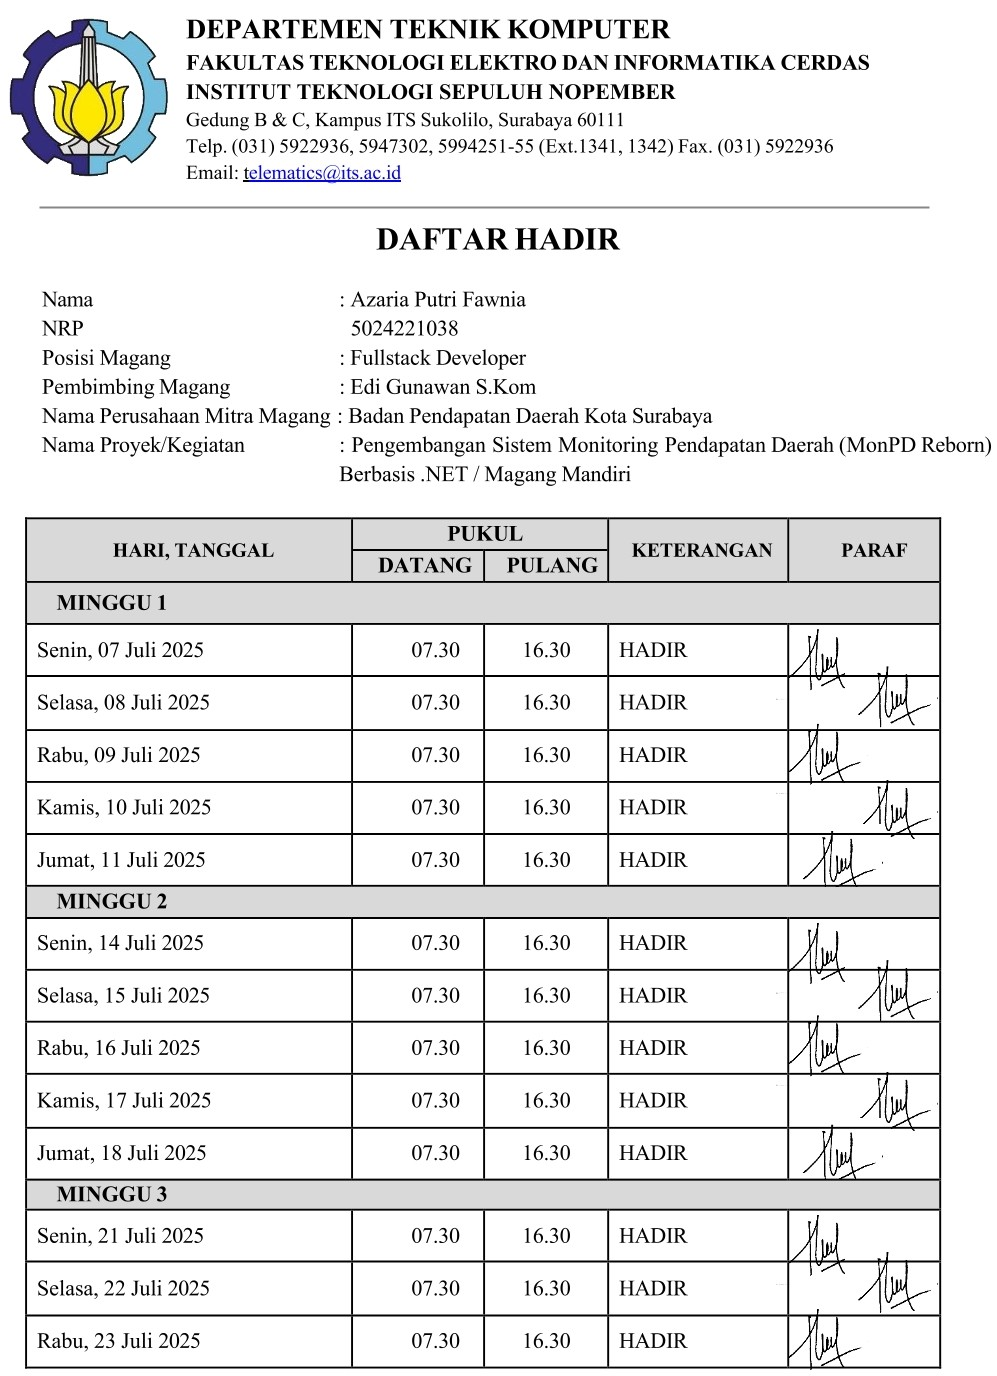
\includegraphics[width=0.99\textwidth]{gambar/Absensi/Absensi-1.jpg} \hfill
    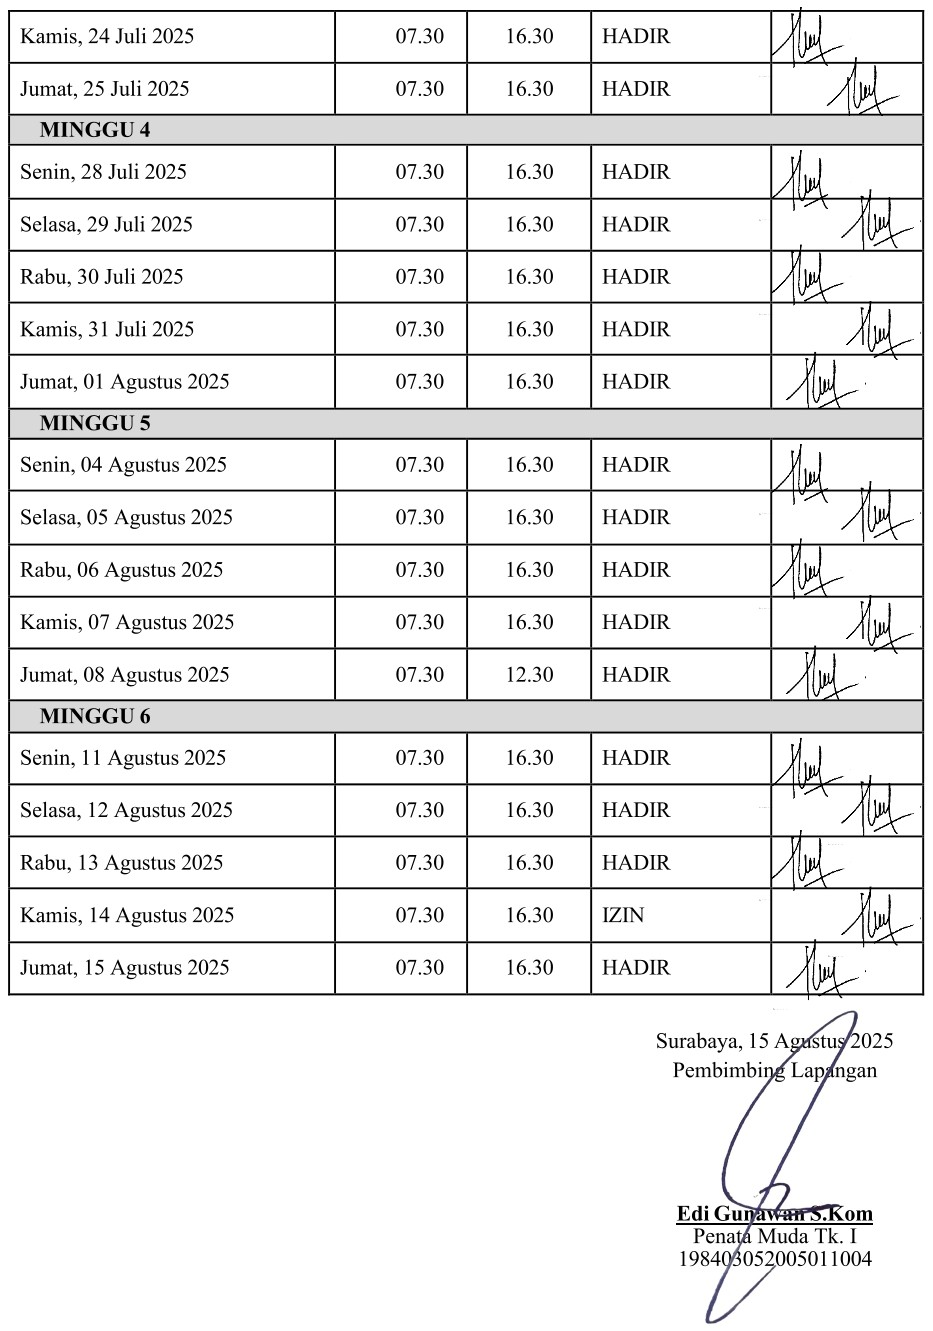
\includegraphics[width=1\textwidth]{gambar/Absensi/Absensi-2.jpg} \hfill
\tutuplampiran